\pdfminorversion=4
\documentclass[aspectratio=169]{beamer}

\mode<presentation>
{
  \usetheme{default}
  \usecolortheme{default}
  \usefonttheme{default}
  \setbeamertemplate{navigation symbols}{}
  \setbeamertemplate{caption}[numbered]
  \setbeamertemplate{footline}[frame number]  % or "page number"
  \setbeamercolor{frametitle}{fg=white}
  \setbeamercolor{footline}{fg=black}
} 

\usepackage[english]{babel}
\usepackage[utf8x]{inputenc}
\usepackage{tikz}
\usepackage{courier}
\usepackage{array}
\usepackage{bold-extra}
\usepackage{minted}
\usepackage[thicklines]{cancel}
\usepackage{fancyvrb}

\xdefinecolor{dianablue}{rgb}{0.18,0.24,0.31}
\xdefinecolor{darkblue}{rgb}{0.1,0.1,0.7}
\xdefinecolor{darkgreen}{rgb}{0,0.5,0}
\xdefinecolor{darkgrey}{rgb}{0.35,0.35,0.35}
\xdefinecolor{darkorange}{rgb}{0.8,0.5,0}
\xdefinecolor{darkred}{rgb}{0.7,0,0}
\definecolor{darkgreen}{rgb}{0,0.6,0}
\definecolor{mauve}{rgb}{0.58,0,0.82}

\title[2018-10-01-dianahep-histbook]{Histogram interoperability}
\author{Jim Pivarski}
\institute{Princeton University -- DIANA-HEP}
\date{October 1, 2018}

\usetikzlibrary{shapes.callouts}

\begin{document}

\logo{\pgfputat{\pgfxy(0.11, 7.4)}{\pgfbox[right,base]{\tikz{\filldraw[fill=dianablue, draw=none] (0 cm, 0 cm) rectangle (50 cm, 1 cm);}\mbox{\hspace{-8 cm}
\includegraphics[height=1 cm]{princeton-logo-long.png}
\includegraphics[height=1 cm]{diana-hep-logo-long.png}}}}}

\begin{frame}
  \titlepage
\end{frame}

\logo{\pgfputat{\pgfxy(0.11, 7.4)}{\pgfbox[right,base]{\tikz{\filldraw[fill=dianablue, draw=none] (0 cm, 0 cm) rectangle (50 cm, 1 cm);}\mbox{\hspace{-8 cm}
\includegraphics[height=1 cm]{princeton-logo.png}
\includegraphics[height=1 cm]{diana-hep-logo.png}}}}}

% Uncomment these lines for an automatically generated outline.
%\begin{frame}{Outline}
%  \tableofcontents
%\end{frame}

% START START START START START START START START START START START START START

\begin{frame}{Histogramming in Python}
\scriptsize
\vspace{0.25 cm}
\begin{columns}
\column{1.1\linewidth}
\renewcommand{\arraystretch}{1.2}
\begin{tabular}{c l c p{2.7 cm} p{1.5 cm} p{4.75 cm}}
pip? & name & last release & interface style & depends on & integrates with \\\hline
& \href{https://root.cern.ch/pyroot}{\textcolor{blue}{PyROOT}} & 2018 & HEP & ROOT & numpy \\
& \href{https://yoda.hepforge.org/pydoc}{\textcolor{blue}{YODA}} & 2018 & HEP & {\it compiled} & matplotlib, yaml \\
$\surd$ & \href{https://pypi.python.org/pypi/physt}{\textcolor{blue}{physt}} & 2018 & HEP + data science & numpy & pandas, xarray, dask, protobuf, matplotlib, vega (plotting), folium (maps) \\
$\surd$ & \href{https://pypi.org/project/fast-histogram}{\textcolor{blue}{fast-histogram}} & 2018 & simple (astronomy) & numpy & \\
$\surd$ & \href{https://pypi.org/project/qhist/}{\textcolor{blue}{qhist}} & 2018 & HEP & ROOT & \\
$\surd$ & \href{https://pypi.org/project/rootpy}{\textcolor{blue}{rootpy}} & 2017 & HEP & ROOT & pytables, matplotlib, stats \\
$\surd$ & \href{https://vaex.io}{\textcolor{blue}{Vaex}} (vaex.io) & 2017 & all-in-one GUI for big data, fast heatmaps & {\it many!} & Jupyter, matplotlib, HDF5, pandas, C++ \\
$\surd$ & \href{https://pypi.python.org/pypi/hdrhistogram}{\textcolor{blue}{hdrhistogram}} & 2017 & ``high dynamic range'' & {\it compiled} & Java, C++ \\
$\surd$ & \href{https://pypi.python.org/pypi/multihist}{\textcolor{blue}{multihist}} & 2017 & numpy wrapper & numpy & matplotlib \\
$\surd$ & \href{https://github.com/ibab/matplotlib-hep}{\textcolor{blue}{matplotlib-hep}} & 2016 & HEP & matplotlib & numpy, scipy \\
$\surd$ & \href{https://pypi.python.org/pypi/pyhistogram}{\textcolor{blue}{pyhistogram}} & 2014 & HEP & numpy & matplotlib, datetime \\
$\surd$ & \href{https://pypi.python.org/pypi/histogram}{\textcolor{blue}{histogram}} & 2011 & HEP & numpy & matplotlib, HDF5 \\
$\surd$ & \href{https://pypi.python.org/pypi/SimpleHist}{\textcolor{blue}{SimpleHist}} & 2011 & HEP & numpy, matplotlib & ROOT \\
$\surd$ & \href{https://pypi.org/project/paida}{\textcolor{blue}{paida}} & 2007 & HEP & & AIDA! \\
& \href{https://github.com/theodoregoetz/histogram}{\textcolor{blue}{theodoregoetz}} & never & HEP & scipy, \mbox{uncertainties} & numpy, matplotlib \\
% $\surd$ & \href{https://pypi.python.org/pypi/histogramy}{\textcolor{blue}{histogramy}} & 2013 & Numpy, Matplotlib, Scikit-Learn & & \\
% $\surd$ & \href{https://pypi.python.org/pypi/pypeaks}{\textcolor{blue}{pypeaks}} & 2014 & & & \\
% $\surd$ & \href{https://pypi.python.org/pypi/hierogram}{\textcolor{blue}{hierogram}} & 2014 & & & \\
% $\surd$ & \href{https://pypi.python.org/pypi/histo}{\textcolor{blue}{histo}} & & & & \\
% $\surd$ & \href{https://pypi.python.org/pypi/python-metrics}{\textcolor{blue}{python-metrics}} & & & & \\
% $\surd$ & \href{https://pypi.python.org/pypi/statscounter}{\textcolor{blue}{statscounter}} & 2016 & & & \\
% $\surd$ & \href{https://pypi.python.org/pypi/datagram}{\textcolor{blue}{datagram}} & & & & \\
% & \href{http://www.ifh.de/~middell/dashi/index.html}{\textcolor{blue}{dashi}} & & & & \\
\end{tabular}
\end{columns}
\end{frame}

\begin{frame}{Over the years, I've written five}
\scriptsize
\vspace{0.25 cm}
\begin{columns}
\column{1.1\linewidth}
\renewcommand{\arraystretch}{1.2}
\begin{tabular}{c l c p{2.7 cm} p{1.5 cm} p{4.75 cm}}
pip? & name & last release & interface style & depends on & integrates with \\\hline
& \href{http://code.google.com/p/plothon}{\textcolor{blue}{Plothon}} & 2006 & HEP & ROOT & SVG \\
& \href{http://code.google.com/p/svgfig}{\textcolor{blue}{SVGFig}} & 2008 & HEP & {\it none!} & SVG \\
& \href{https://github.com/opendatagroup/cassius}{\textcolor{blue}{Cassius}} & 2013 & HEP + data science & numpy & SVG, Augustus (Open Data Group) \\
$\surd$ & \href{https://github.com/histogrammar}{\textcolor{blue}{Histogrammar}} & 2016 & combinational library & numpy & Spark, Julia, CUDA, \mbox{ROOT (Cling),} matplotlib, Bokeh, Vega \\
$\surd$ & \href{https://github.com/scikit-hep/histbook}{\textcolor{blue}{histbook}} & 2018 & HEP & numpy & Spark, Pandas, Vega \\
\end{tabular}
\end{columns}

\large
\begin{uncoverenv}<2->
\vspace{1 cm}
\underline{\it Implementing} data analysis tools isn't the problem, it's designing the \underline{\it right} tool, one that solves the Cuisinart Problem:

\begin{center}
\begin{minipage}{0.8\linewidth}
It slices and dices, but is it worth the setup and cleanup?
\end{minipage}
\end{center}

Experimentation in this area is valuable.
\end{uncoverenv}
\end{frame}

\begin{frame}{All these libraries are overwhelming!}
\large
\vspace{0.5 cm}
\begin{center}

\includegraphics[width=0.4\linewidth]{standards.png}
\end{center}

\vspace{0.5 cm}
However, the problem isn't that data analysts are using different tools; the problem is communicating results between them.
\end{frame}

\begin{frame}{There is a standard: ROOT files}
\large
\vspace{0.5 cm}
Even if the point of a tool is to work in a non-ROOT way or to avoid ROOT dependencies, we can still share results using the ROOT file format.

\vspace{1 cm}
\textcolor{darkblue}{Look at industry:}
\begin{itemize}
\item dozens of big data SQL engines that all run on Parquet files;
\item dozens of machine learning tools that all run on Numpy from HDF5 files.
\end{itemize}

\vspace{0.25 cm}
The most conservative part of a software ecosystem is its persistence format.

\vspace{1 cm}
ROOT files are incredibly well established in HEP. It would take a strong technical argument/corner case to use something else.
\end{frame}

\begin{frame}[fragile]{Writing histograms with uproot}
\large
\vspace{0.5 cm}
uproot version 3 has write support, but (currently) only for histograms.

\small
\begin{minted}{python}
>>> import uproot
>>> import numpy
>>> f = uproot.recreate("tmp.root")
>>> f["name"] = numpy.histogram(numpy.random.normal(0, 1, 100000))
\end{minted}

\vspace{1 cm}
\large
Read it back in ROOT:

\small
\begin{minted}{python}
>>> import ROOT
>>> f = ROOT.TFile("tmp.root")
>>> h = f.Get("name")
>>> h.Draw()
\end{minted}

\vspace{-3.5 cm}
\hfill 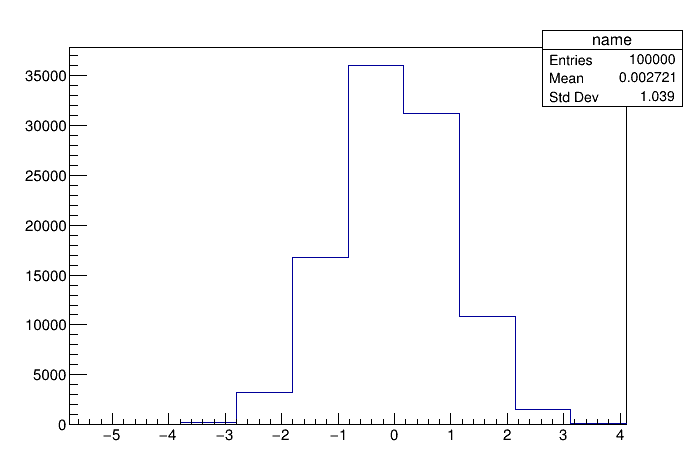
\includegraphics[width=0.5\linewidth]{root-hist.png}
\end{frame}

\begin{frame}[fragile]{Bidirectional conversions to and from many libraries}
\vspace{0.1 cm}
\normalsize
Save a Physt plot to a ROOT file:

\small
\begin{minted}{python}
>>> import physt
>>> f = uproot.recreate("tmp.root")
>>> f["name"] = physt.h1(numpy.random.normal(0, 1, 100000), bins=16,
...                      range=(-4, 4), name="physt histogram")
\end{minted}

\normalsize
Read it back as Physt:

\small
\begin{minted}{python}
>>> f["name"].physt().plot()
\end{minted}

\normalsize
Read it back as a Numpy contents-and-edges tuple:

\small
\begin{minted}{python}
>>> f["name"].numpy()
\end{minted}

\tiny
\begin{verbatim}
(array([   23,   112,   473,  1652,  4370,  9061, 15024, 19213, 19091, 15019,  9128,  4501,  1671,   512,   128,    16], dtype=int32),
 array([-4. , -3.5, -3. , -2.5, -2. , -1.5, -1. , -0.5,  0. ,  0.5,  1. ,  1.5,  2. ,  2.5,  3. ,  3.5,  4. ]))
\end{verbatim}

\normalsize
Read it in ROOT:

\small
\begin{minted}{python}
>>> f = ROOT.TFile("tmp.root")
>>> h = f.Get("name")
>>> h.Draw()
\end{minted}
\end{frame}

\begin{frame}[fragile]{Not really ``histograms:'' HEPData archival format (YAML)}
\small
\begin{minted}{python}
>>> print(f["name"].hepdata())
\end{minted}

\tiny
\vspace{-0.6 cm}
\begin{columns}[t]
\column{0.4\linewidth}
\begin{verbatim}
independent_variables:
- header: {name: physt histogram, units: null}
  values:
  - {low: -4.0, high: -3.5}
  - {low: -3.5, high: -3.0}
  - {low: -3.0, high: -2.5}
  - {low: -2.5, high: -2.0}
  - {low: -2.0, high: -1.5}
  - {low: -1.5, high: -1.0}
  - {low: -1.0, high: -0.5}
  - {low: -0.5, high: 0.0}
  - {low: 0.0, high: 0.5}
  - {low: 0.5, high: 1.0}
  - {low: 1.0, high: 1.5}
  - {low: 1.5, high: 2.0}
  - {low: 2.0, high: 2.5}
  - {low: 2.5, high: 3.0}
  - {low: 3.0, high: 3.5}
  - {low: 3.5, high: 4.0}
dependent_variables:
- header: {name: counts, units: null}
  qualifiers: []
  values:
  - value: 23.0
    errors:
    - {symerror: 4.795831523312719, label: stat}
  - value: 112.0
    errors:
    - {symerror: 10.583005244258363, label: stat}
\end{verbatim}
\column{0.5\linewidth}
\begin{verbatim}
  - value: 473.0
    errors:
    - {symerror: 21.748563170931547, label: stat}
  - value: 1652.0
    errors:
    - {symerror: 40.64480286580315, label: stat}
  - value: 4370.0
    errors:
    - {symerror: 66.10597552415364, label: stat}
  - value: 9061.0
    errors:
    - {symerror: 95.1892851112981, label: stat}
  - value: 15024.0
    errors:
    - {symerror: 122.5724275683565, label: stat}
  - value: 19213.0
    errors:
    - {symerror: 138.61096637712328, label: stat}
  - value: 19091.0
    errors:
    - {symerror: 138.17018491700733, label: stat}
  - value: 15019.0
    errors:
    - {symerror: 122.55202976695246, label: stat}
  - value: 9128.0
    errors:
    - {symerror: 95.5405672999695, label: stat}
  - value: 4501.0
    errors:
    - {symerror: 67.08949247087803, label: stat}
  - value: 1671.0
    errors:
    - {symerror: 40.87786687193939, label: stat}
  - value: 512.0
    errors:
    - {symerror: 22.627416997969522, label: stat}
  - value: 128.0
    errors:
    - {symerror: 11.313708498984761, label: stat}
  - value: 16.0
    errors:
    - {symerror: 4.0, label: stat}
\end{verbatim}
\end{columns}
\end{frame}

\begin{frame}[fragile]{Not really ``histograms:'' Pandas DataFrame}
\large

\begin{columns}[b]
\column{0.4\linewidth}
\small
\begin{minted}{python}
>>> f["name"].pandas()
\end{minted}

\scriptsize
\begin{verbatim}
                 count  variance
physt histogram
[-inf, -4.0)         5         5
[-4.0, -3.5)        23        23
[-3.5, -3.0)       112       112
[-3.0, -2.5)       473       473
[-2.5, -2.0)      1652      1652
[-2.0, -1.5)      4370      4370
[-1.5, -1.0)      9061      9061
[-1.0, -0.5)     15024     15024
[-0.5, 0.0)      19213     19213
[0.0, 0.5)       19091     19091
[0.5, 1.0)       15019     15019
[1.0, 1.5)        9128      9128
[1.5, 2.0)        4501      4501
[2.0, 2.5)        1671      1671
[2.5, 3.0)         512       512
[3.0, 3.5)         128       128
[3.5, 4.0)          16        16
[4.0, inf)           1         1
\end{verbatim}

\column{0.45\linewidth}
The index for this DataFrame is an {\tt\normalsize IntervalIndex}.

\vspace{0.5 cm}
The {\tt\normalsize variance} column is the ``sumw2'' (identical to count when filled without weights).

\vspace{0.5 cm}
There's room here for profile plots to share the same binning.

\vspace{0.5 cm}
See the F.A.S.T.\ package for CMS: Ben Krikler and Tai Sakuma.

\vspace{0.5 cm}
\end{columns}
\end{frame}

\begin{frame}{We can add more without upsetting uproot}
\large
\vspace{0.5 cm}
The code that understands streamers and how to write a TH1 is in {\bf uproot}.

\vspace{0.5 cm}
The code that understands how to convert to and from other libraries is in {\bf uproot-methods}. We can make changes to {\bf uproot-methods} independently of (and more rapidly than) {\bf uproot}.

\begin{center}
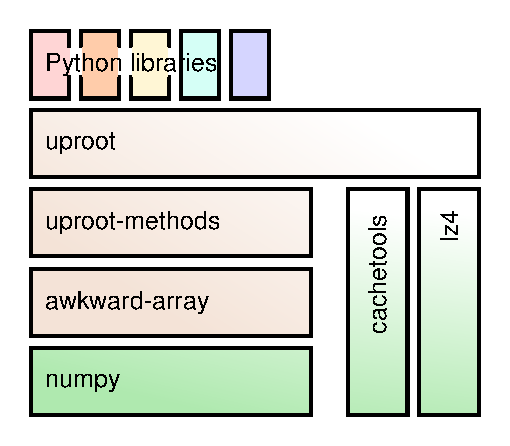
\includegraphics[width=0.4\linewidth]{abstraction-layers.pdf}
\end{center}
\end{frame}

\begin{frame}{What about Histogrammar and histbook?}
\vspace{0.25 cm}
\begin{center}

\includegraphics[width=0.55\linewidth]{histogrammar-logo-paths.pdf}

\vspace{1 cm}

\includegraphics[width=0.45\linewidth]{histbook-logo.pdf}
\end{center}
\end{frame}

\begin{frame}[fragile]{Histogrammar}
\large
\vspace{0.5 cm}
Redesigned histogramming as a combinational library: you put simple pieces together to build n-dimensional histograms and profiles.

\vspace{1 cm}

\begin{columns}[t]
\column{0.47\linewidth}
\small
\textcolor{darkblue}{\normalsize Histograms:}
\begin{minted}{python}
Bin(num, low, high, fillRule,
  Count())
\end{minted}

\vspace{0.25 cm}
\textcolor{darkblue}{\normalsize Three-dimensional histograms:}
\begin{minted}{python}
Bin(xnum, xlow, xhigh, xfill,
  Bin(ynum, ylow, yhigh, yfill,
    Bin(znum, zlow, zhigh, zfill,
      Count()))
\end{minted}

\column{0.5\linewidth}
\textcolor{darkblue}{\normalsize Profile plots:}
\small
\begin{minted}{python}
Bin(xnum, xlow, xhigh, xfill,
  Deviate(yfill))
\end{minted}

{\small where {\ttfamily\small Deviate} aggregates a mean and standard deviation.}

\vspace{0.25 cm}
\textcolor{darkblue}{\normalsize Mix and match binning methods:}
\small
\begin{minted}{python}
SparselyBin(0.01, filleta,
  Bin(314, -3.14, 3.14, fillphi,
    Count()))
\end{minted}
\end{columns}
\end{frame}

\begin{frame}{Histogrammar}
\large
\vspace{0.5 cm}
But it was too general. An arbitrary tree of aggregators produces an arbitrary tree of aggregated data, which is hard to format as a plot.

\vspace{1 cm}
The cartesian grid of axis types and storage types in Boost-Histogram and ROOT~7 histograms (and histbook) is general enough.
\end{frame}

\begin{frame}[fragile]{histbook: the ``hist'' part}
\vspace{0.1 cm}
Make cartesian, n-dimensional histograms that you can assign to plot facets on the fly.

\scriptsize
\begin{onlyenv}<1>
\scriptsize
\begin{minted}{python}
>>> from histbook import *
>>> multihist = Hist(bin("mass", 100, 0, 500), cut("q1*q2 < 0"),
...                  split("mt1", [0.2, 0.5]), split("mt2", [0.2, 0.5]), fill=df)
>>> multihist.step("mass")
\end{minted}
\mbox{ } \hfill 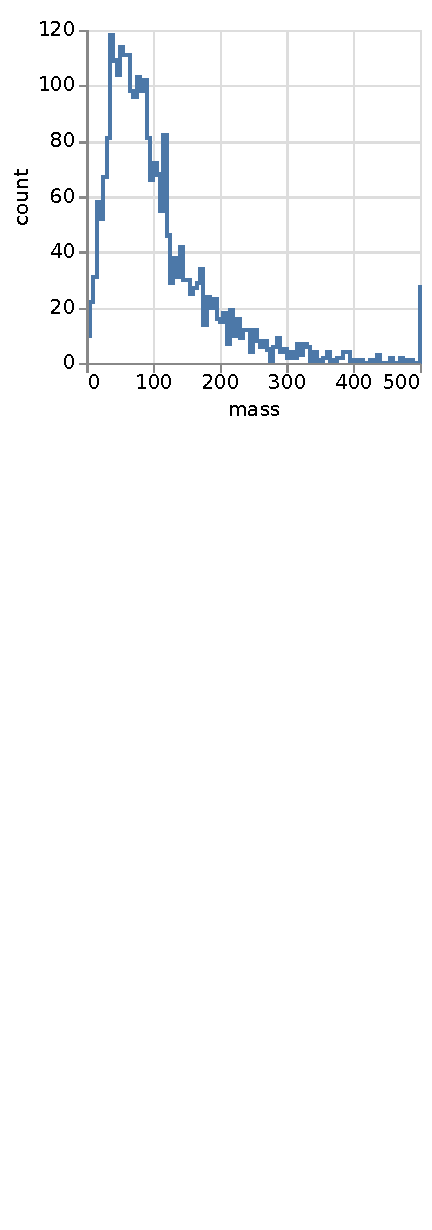
\includegraphics[height=6 cm]{pandhist.pdf} \hfill \mbox{ }
\end{onlyenv}
\begin{onlyenv}<2>
\scriptsize
\begin{minted}{python}
>>> from histbook import *
>>> multihist = Hist(bin("mass", 100, 0, 500), cut("q1*q2 < 0"),
...                  split("mt1", [0.2, 0.5]), split("mt2", [0.2, 0.5]), fill=df)
>>> multihist.overlay("q1*q2 < 0").step("mass")
\end{minted}
\mbox{ } \hfill 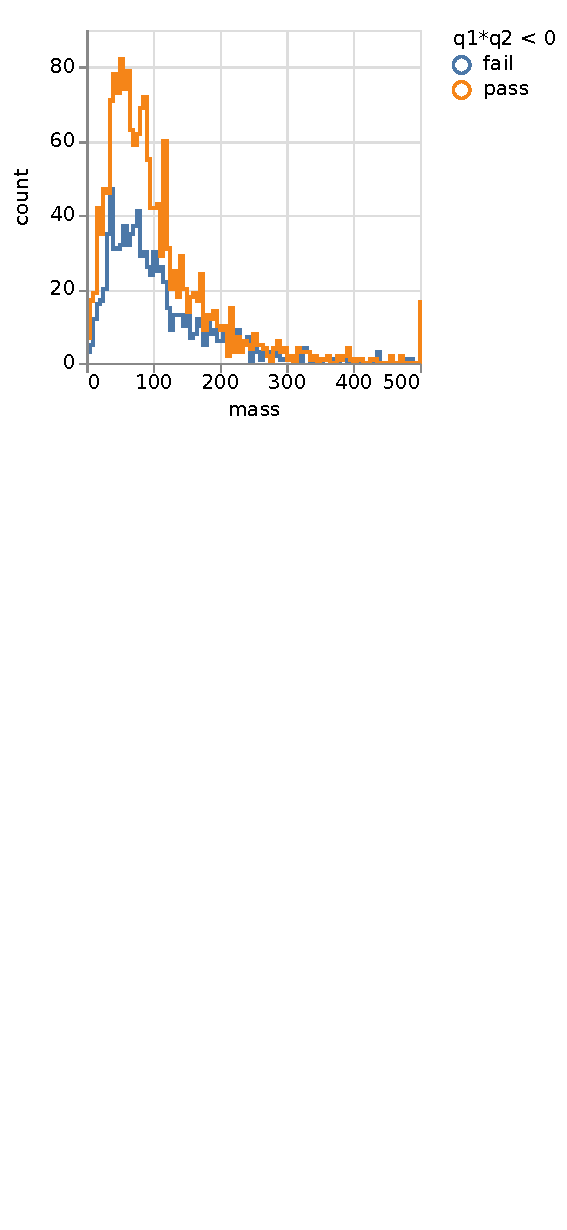
\includegraphics[height=6 cm]{pandhist_overlay.pdf} \hfill \mbox{ }
\end{onlyenv}
\begin{onlyenv}<3>
\scriptsize
\begin{minted}{python}
>>> from histbook import *
>>> multihist = Hist(bin("mass", 100, 0, 500), cut("q1*q2 < 0"),
...                  split("mt1", [0.2, 0.5]), split("mt2", [0.2, 0.5]), fill=df)
>>> multihist.stack("q1*q2 < 0").area("mass")
\end{minted}
\mbox{ } \hfill 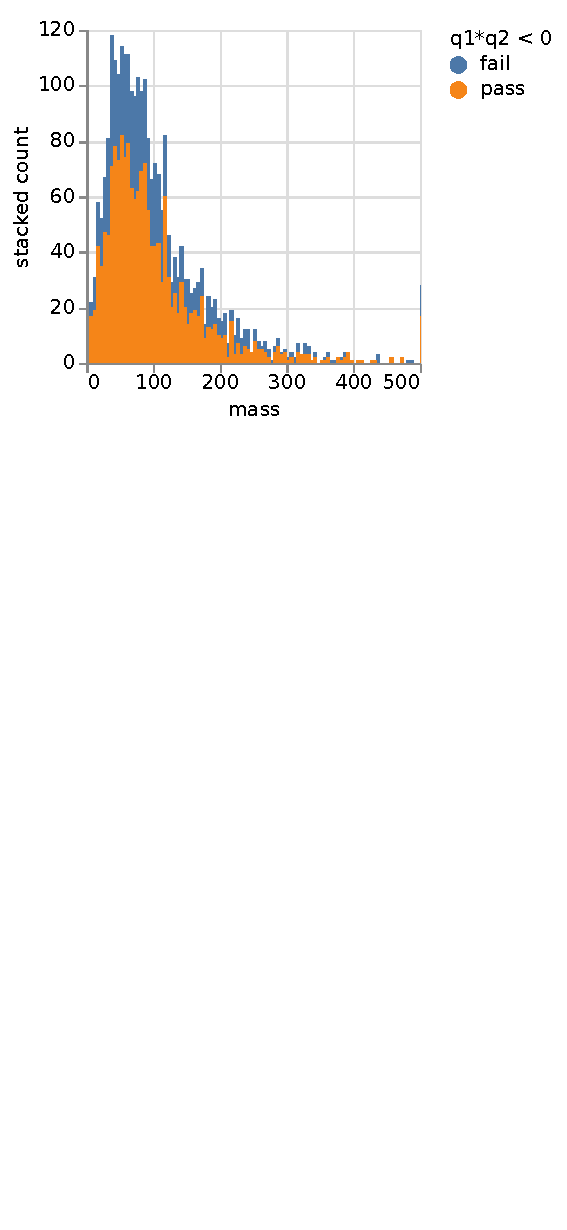
\includegraphics[height=6 cm]{pandhist_stack.pdf} \hfill \mbox{ }
\end{onlyenv}
\begin{onlyenv}<4>
\scriptsize
\begin{minted}{python}
>>> from histbook import *
>>> multihist = Hist(bin("mass", 100, 0, 500), cut("q1*q2 < 0"),
...                  split("mt1", [0.2, 0.5]), split("mt2", [0.2, 0.5]), fill=df)
>>> multihist.beside("q1*q2 < 0").step("mass")
\end{minted}
\mbox{ } \hfill 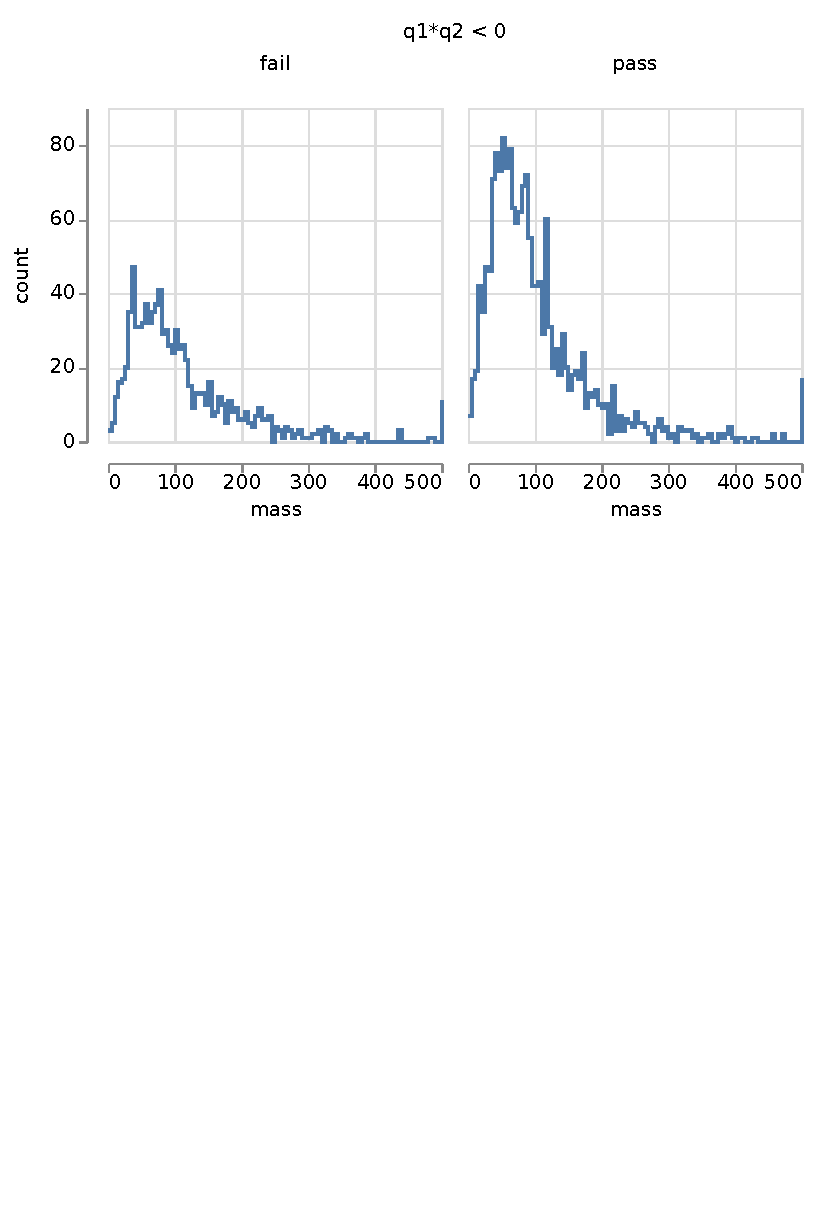
\includegraphics[height=6 cm]{pandhist_trellis.pdf} \hfill \mbox{ }
\end{onlyenv}
\begin{onlyenv}<5>
\scriptsize
\begin{minted}{python}
>>> from histbook import *
>>> multihist = Hist(bin("mass", 100, 0, 500), cut("q1*q2 < 0"),
...                  split("mt1", [0.2, 0.5]), split("mt2", [0.2, 0.5]), fill=df)
>>> multihist.below("mt1").beside("mt2").step("mass")
\end{minted}
\mbox{ } \hfill 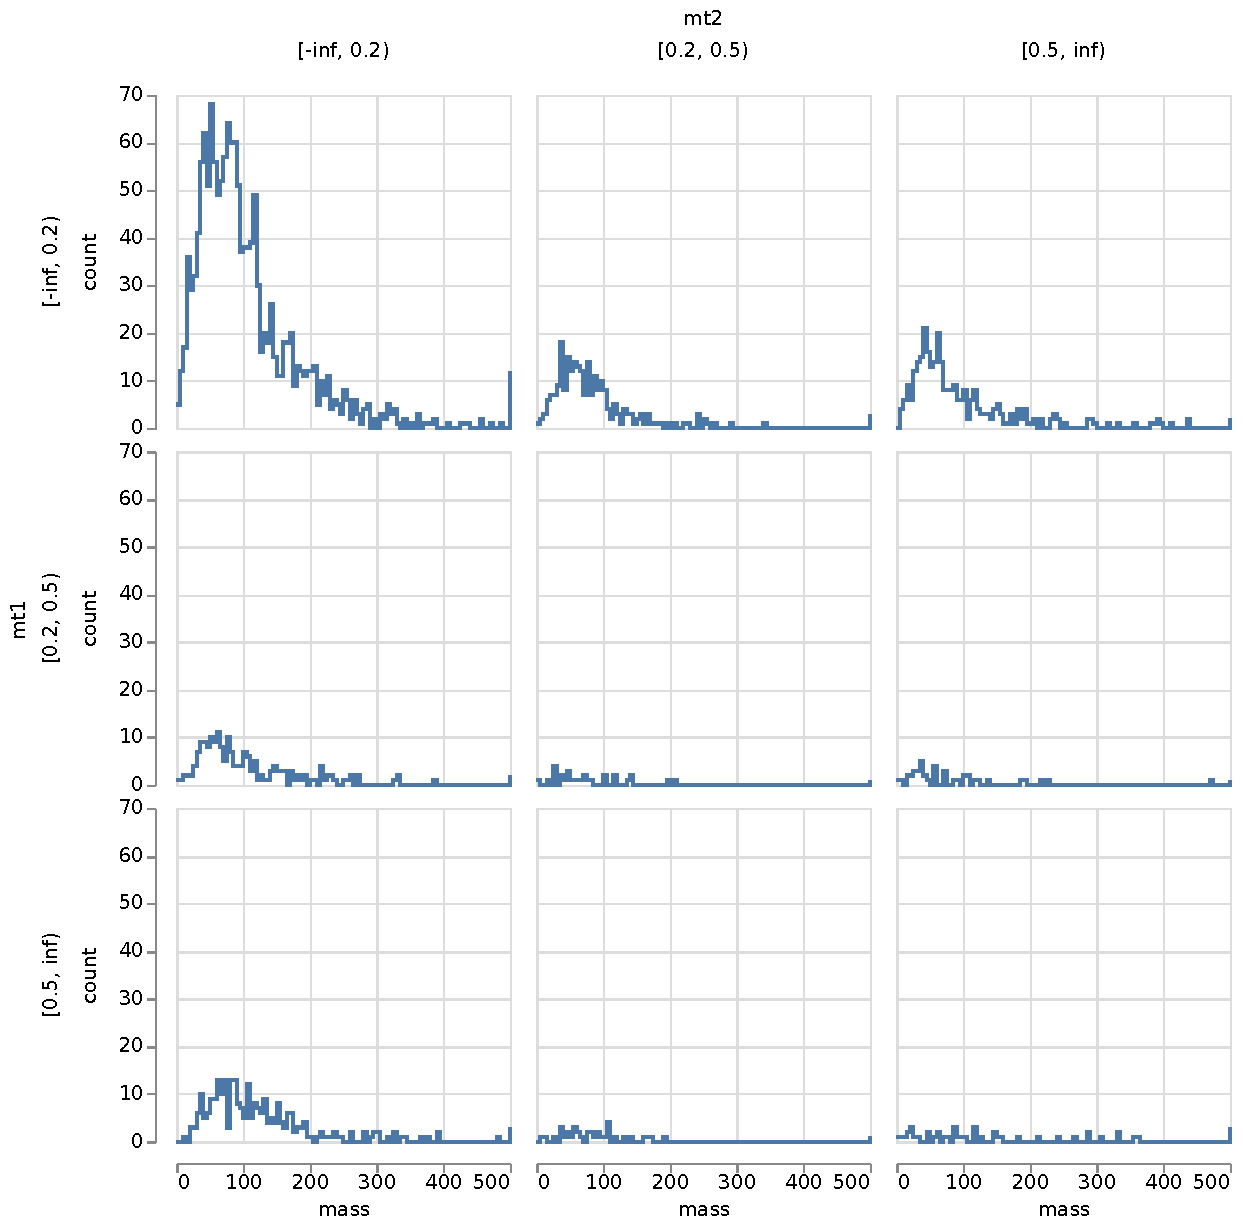
\includegraphics[height=6 cm]{pandhist_double_trellis.pdf} \hfill \mbox{ }
\end{onlyenv}
\begin{onlyenv}<6>
\scriptsize
\begin{minted}{python}
>>> from histbook import *
>>> multihist = Hist(bin("mass", 100, 0, 500), cut("q1*q2 < 0"),
...                  split("mt1", [0.2, 0.5]), split("mt2", [0.2, 0.5]), fill=df)
>>> multihist.below("mt1").beside("mt2").overlay("q1*q2 < 0").step("mass")
\end{minted}
\mbox{ } \hfill 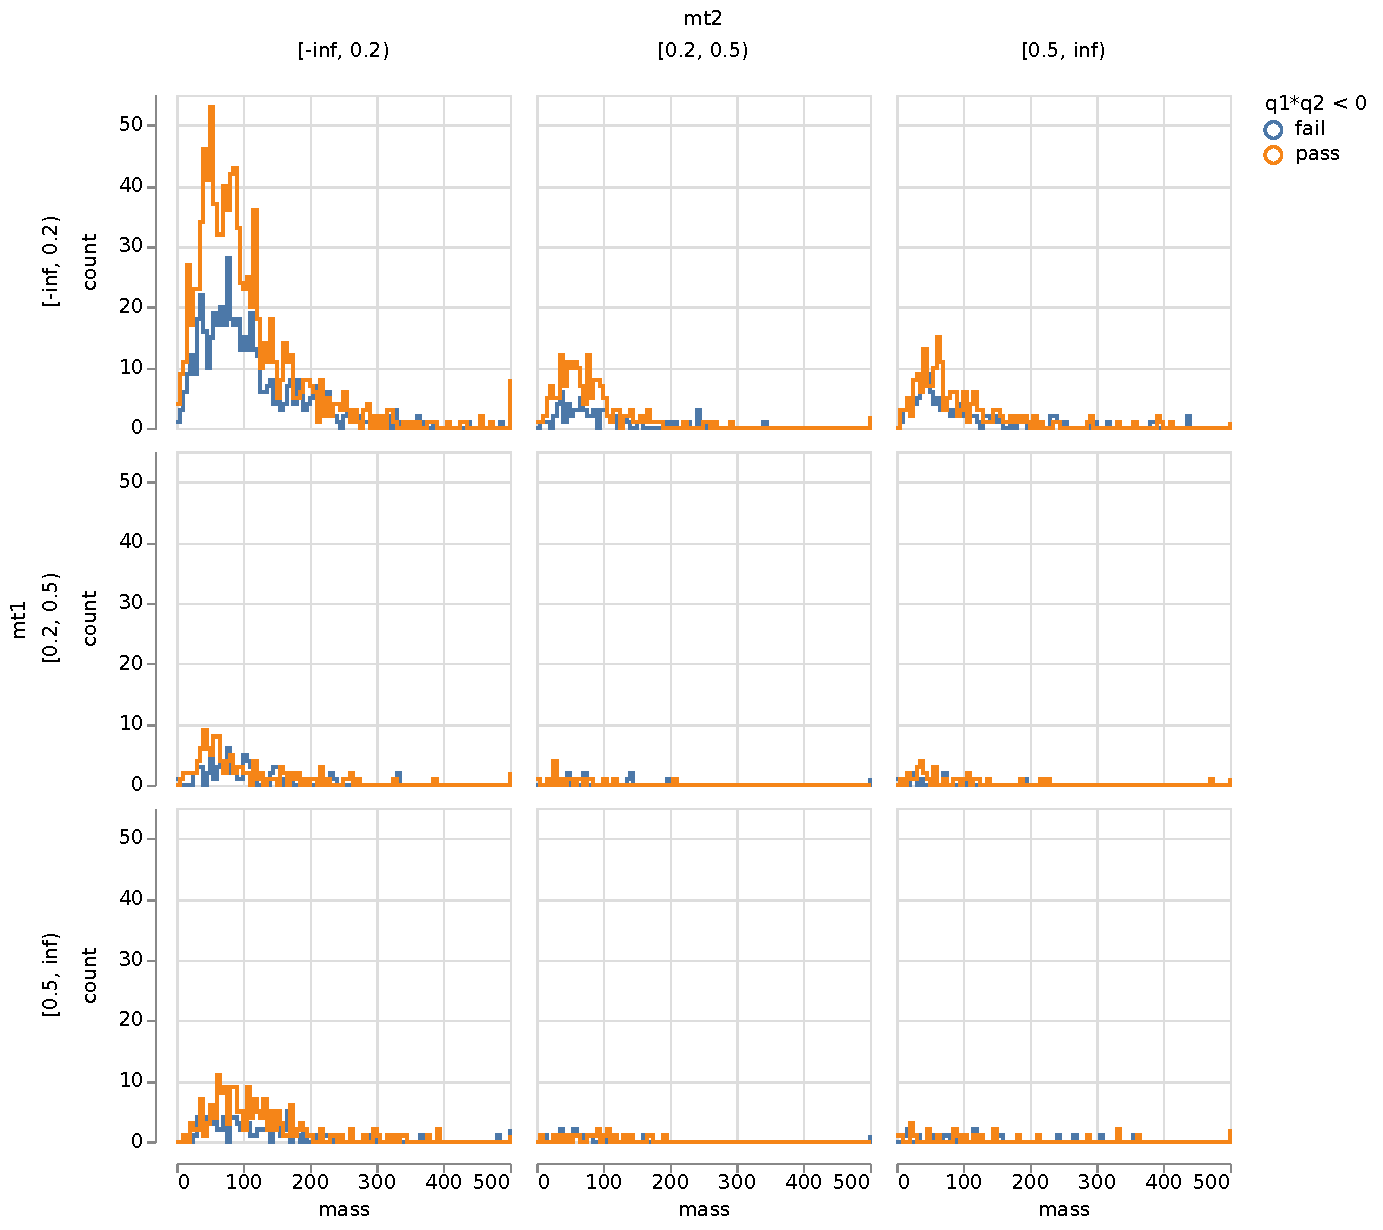
\includegraphics[height=6 cm]{pandhist_double_trellis_overlay.pdf} \hfill \mbox{ }
\end{onlyenv}
\end{frame}

\begin{frame}{histbook: the ``book'' part}
\vspace{0.5 cm}
\textcolor{darkblue}{Problem:} physicists define semantic relationships between a large set (thousands) of histograms three or four times:
\begin{enumerate}
\item when they construct the histograms (defining the binning)
\item when they fill the histograms
\item when they fit with CMS Conbine or ATLAS HistFactory
\item when they publish results on HEPData
\end{enumerate}

\vspace{0.5 cm}
\textcolor{darkblue}{Solution to 1--2:} use functional programming to put the ``fill rule'' next to the binning: Histogrammar, histbook, and RDataFrame.
\end{frame}

\begin{frame}[fragile]{histbook: the ``book'' part}
\vspace{0.25 cm}
\textcolor{darkblue}{Solution to 2--3--4?:} declare trees of related histograms and communicate this relationship to fitters:

\scriptsize
\begin{minted}{python}
everything = ChannelsBook(
    mass = SamplesBook(["data", "signal", "background"],
                  SystematicsBook(Hist(bin("x", 5, 0, 5), systematic=[0]),
                                  Hist(bin("x + epsilon", 5, 0, 5), systematic=[1]),
                                  Hist(bin("x - epsilon", 5, 0, 5), systematic=[-1]))),
    truth = SamplesBook(["signal", "background"],
                        Book(par1=Hist(bin("par1", 5, 0, 5)),
                             par2=Hist(bin("par2", 5, 0, 5)))))
\end{minted}

\normalsize
\vspace{0.5 cm}
A {\tt\small Book} has a fill method like {\tt\small Hist}, so these collections of histograms can be filled in one pass and retain their internal relationships, to be reused for fitting.

\vspace{0.5 cm}
This is research: what's the right way to structure histograms for fitting that still makes sense for filling? Need to work with developers of fitting libraries.
\end{frame}

\begin{frame}[fragile]{Third idea: Pandas DataFrames should be histograms}
\vspace{-0.25 cm}
A DataFrame with an {\tt\normalsize IntervalIndex} is a {\it sparse} histogram.

\scriptsize
\vspace{-0.35 cm}
\begin{verbatim}
             one                  two                 three
----------------     ----------------     -----------------
[0.0, 1.0)  4538     [1.0, 2.0)    71     [6.0, 7.0)     41
[1.0, 2.0)  4513     [2.0, 3.0)  5009     [7.0, 8.0)   4708
[2.0, 3.0)   483     [3.0, 4.0)  4868
[3.0, 4.0)     4     [4.0, 5.0)    52
\end{verbatim}

\normalsize
\vspace{-0.35 cm}
\begin{uncoverenv}<2->
Adding and other operations would just ``do the right thing'' if not for frustrating details like imputing NaN when an interval key is missing, rather than zero.

\scriptsize
\begin{minted}{python}
>>> def add(*args):
...     return reduce(lambda x, y: x.add(y, fill_value=0), args)
\end{minted}

\scriptsize
\vspace{-0.35 cm}
\begin{verbatim}
   add(one, two)      add(two, three)     add(one, two, three)
----------------     ----------------     --------------------
[0.0, 1.0)  4538     [1.0, 2.0)    71     [0.0, 1.0)      4538
[1.0, 2.0)  4584     [2.0, 3.0)  5009     [1.0, 2.0)      4584
[2.0, 3.0)  5492     [3.0, 4.0)  4868     [2.0, 3.0)      5492
[3.0, 4.0)  4872     [4.0, 5.0)    52     [3.0, 4.0)      4872
[4.0, 5.0)    52     [6.0, 7.0)    41     [4.0, 5.0)        52
                     [7.0, 8.0)  4708     [6.0, 7.0)        41
                                          [7.0, 8.0)      4708
\end{verbatim}

\vspace{-2 cm}
\large
\hfill Wrap it \mbox{as\hspace{0.3 cm}}

\hfill a subclass?
\end{uncoverenv}
\end{frame}

\begin{frame}{Conclusions}
\Large
\vspace{0.25 cm}
\begin{itemize}\setlength{\itemsep}{0.25 cm}
\item The design of data analysis tools like histogramming has an impact on human efficiency. It's worth optimizing (experimentally).
\item The chaos of different tools can be mitigated by a common persistence format, and ROOT's the leading candidate.
\item Some of the ideas in Histogrammar and histbook are also in Boost-Histogram, Physt, and ROOT 7. Some aren't. I'd rather contribute ideas than maintain my own library.
\item Looking forward to finding ways to collaborate, get feedback from users, and iterate.
\end{itemize}
\end{frame}

\end{document}
